% 1 · Statement and problem
\section{Statement and problem}

\begin{frame}{AI runs on physical infrastructure, and it is growing fast}
  Every AI model runs in a data centre that draws electricity, uses water for cooling, and is
  built from mined hardware that ends as e-waste.
  \vspace{14pt}

  \centering
  \bignum{$\approx$1.5\%}{of world electricity used by\\data centres (2024)}\hfill
  \bignum{$\approx$2×}{by 2030: 415 → 945 TWh\\(IEA base case)}\hfill
  \bignum{7 of 9}{planetary boundaries\\already transgressed (2025)}
  \src{IEA (2025) \emph{Energy and AI}; Sakschewski et al.\ (2025) \emph{Planetary Health Check}}
  \note{%
    \NoteKey{AI is physical, and the electricity it needs is about to double.}
    \NoteSlide{Three numbers. $\approx$1.5\%: data centres' share of world electricity in 2024 (415 TWh). $\approx$2$\times$:
    the IEA's projection of 945 TWh by 2030. 7 of 9: planetary boundaries assessed as crossed in 2025.}
    \NoteWhy{1.5\% sounds small. The point of the whole talk is that it is not spread evenly.}
    \NoteSay{40}{Every time someone uses an AI model, a data centre somewhere draws electricity, evaporates water to cool
    its chips, and runs on hardware made from mined minerals. Data centres used about 1.5\% of the world's electricity
    in 2024, and the International Energy Agency expects that to roughly double by 2030. And this growth lands on a
    planet that has already crossed seven of its nine boundaries.}
    \begin{NoteAsk}
      \item \emph{Is 945 TWh measured?} No: it is the IEA's base-case projection for 2030.
    \end{NoteAsk}
  }
\end{frame}

\begin{frame}{Seven of nine planetary boundaries are now crossed}
  \centering
  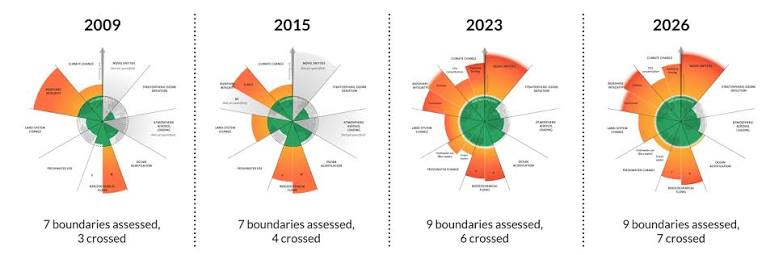
\includegraphics[width=.9\textwidth]{pics/pb_trangression.png}\par
  \vspace{6pt}\raggedright\small
  Each assessment has found more boundaries crossed: from 3 in 2009 to 7 today. AI data centres press on
  several of them: climate through electricity (O1); freshwater, novel entities and biosphere
  integrity through cooling water, e-waste and mining (O2).
  \src{Graphic: Stockholm Resilience Centre, \emph{Planetary boundaries} (stockholmresilience.org). Assessments: Rockström et al.\ (2009); Steffen et al.\ (2015); Richardson et al.\ (2023); Planetary Health Check.}
  \note{%
    \NoteKey{The planet is already outside most of its safe limits, so any new pressure matters.}
    \NoteSlide{The Stockholm Resilience Centre's charts for 2009, 2015, 2023 and 2026. Each wedge is one boundary: the green
    centre is the safe zone, orange to red means crossed. The count rose from 3 crossed (of 7 assessed) to 7 (of 9).}
    \NoteWhy{It sets the frame for the talk: which of these boundaries do AI data centres press on, and at what scale?}
    \NoteSay{30}{The planetary-boundaries framework sets nine limits on how far we can push the Earth system before risking
    abrupt change. Every new assessment has found more of them crossed: three in 2009, seven today. Our question is which
    of these AI data centres press on: climate through their electricity, freshwater through cooling and power plants,
    and novel entities and the biosphere through e-waste and mining. We come back to this as a matrix at the end.}
    \begin{NoteAsk}
      \item \emph{Did data centres cause this?} No. This is a global assessment of all human activity; we only map AI's
        pathways onto it.
    \end{NoteAsk}
  }
\end{frame}

\begin{frame}{Small globally, but highly concentrated}
  \begin{itemize}\footnotesize
    \item The US (45\%), China (25\%) and Europe (15\%) use 85\% of data-centre electricity (415 TWh, 2024);
      tracked AI capacity is even more concentrated: 83\% of 15 GW is in the US
    \item So impacts fall on particular \textbf{grids, basins and communities}. One quarter of data centres sit in
      water-stressed areas, but that count ignores \textbf{size} and \textbf{water use}
  \end{itemize}
  \centering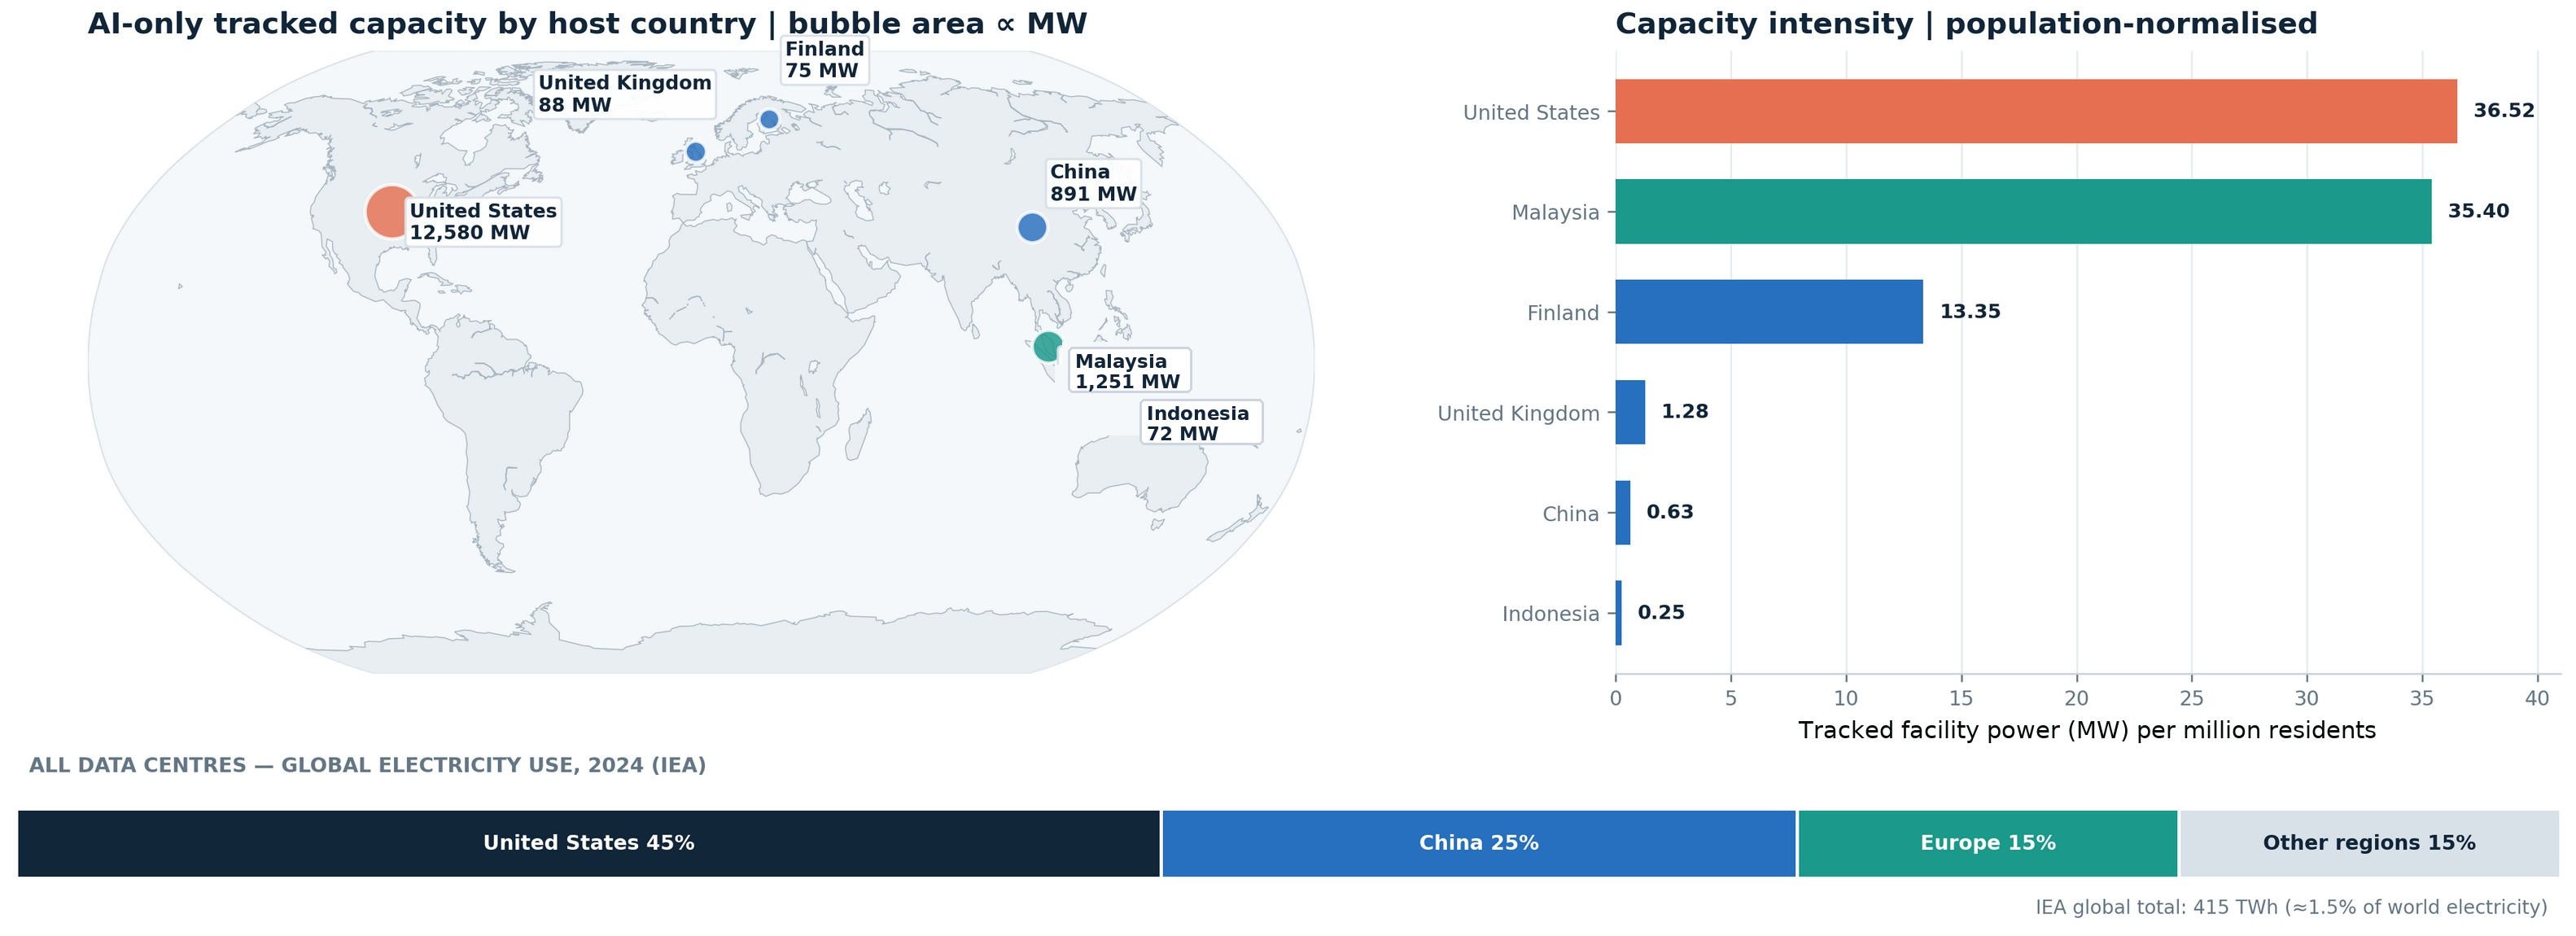
\includegraphics[width=.8\textwidth]{pics/aditya/capacity_map_crop.png}
  \src{IEA (2025) \emph{Energy and AI}; Epoch AI (2026); UN DESA \emph{World Population Prospects 2024}; Rosa et al.\ (2026). Two denominators: IEA covers all data-centre electricity; Epoch covers tracked AI sites only.}
  \note{%
    \NoteKey{Data-centre electricity, and AI capacity even more, sits in very few countries.}
    \NoteSlide{Left map: bubbles show tracked AI data-centre capacity by country (US 12,580 MW, Malaysia 1,251, China 891).
    Right bars: capacity per million residents; the US and Malaysia are far ahead. Bottom bar: the IEA's split of
    \emph{all} data-centre electricity: US 45\%, China 25\%, Europe 15\%.}
    \NoteWhy{Two different datasets, same message. The IEA covers all data centres; Epoch AI covers 96 large AI sites.}
    \NoteSay{45}{Globally data centres are small, but they are concentrated. Three regions, the US, China and Europe, use
    85\% of data-centre electricity. For AI capacity it is even more extreme: 83\% of the 15 gigawatts we track is in the
    US. So the impacts fall on particular grids, basins and communities. A 2026 study found that a quarter of data
    centres sit in water-stressed areas, but it counts sites, not their size or water use. That is the gap we fill.}
    \begin{NoteAsk}
      \item \emph{Why is Malaysia so high per person?} Several large AI sites in Johor, next to Singapore, and a small
        population.
    \end{NoteAsk}
  }
\end{frame}

\begin{frame}{Three phases since 1950, and one puzzle}
  \centering
  \begin{tikzpicture}[x=1cm,y=1cm]
    \fill[phaseGA]    (0,0)    rectangle (6.4,.75) node[midway,white,font=\scriptsize\bfseries] {Great Acceleration · 1950–2010};
    \fill[phaseCloud] (6.45,0) rectangle (10.0,.75) node[midway,white,font=\scriptsize\bfseries] {Cloud era · 2010–2018};
    \fill[phaseAI]    (10.05,0) rectangle (13.6,.75) node[midway,white,font=\scriptsize\bfseries] {AI era · 2019 →};
    \node[below,font=\scriptsize,text width=6cm,align=center]   at (3.2,-.05)  {Energy, CO\textsubscript{2} and materials rise together};
    \node[below,font=\scriptsize,text width=3.4cm,align=center] at (8.22,-.05) {Compute +550\%, electricity +6\% (2010–18)};
    \node[below,font=\scriptsize,text width=3.4cm,align=center] at (11.82,-.05){US data centres 76 → 176 TWh (2018–2023)};
  \end{tikzpicture}
  \vspace{22pt}

  {\large\bfseries Why did cloud growth leave energy use almost flat,\\
  while AI growth does not?\par}
  \vspace{10pt}
  {\scriptsize\color{muted} In this project, \emph{AI} means data-centre infrastructure.\par}
  \src{Masanet et al.\ (2020) \emph{Science}; Shehabi et al.\ (2024) LBNL; Steffen et al.\ (2015)}
  \note{%
    \NoteKey{Data centres grew for years with little extra energy; AI broke that pattern.}
    \NoteSlide{A timeline of three phases with one fact each. Great Acceleration: energy, CO\textsubscript{2} and materials
    rise together. Cloud era: compute instances +550\% but electricity only +6\% (2010--18). AI era: US data-centre
    electricity 76 $\to$ 176 TWh (2018--2023).}
    \NoteWhy{This is the puzzle the talk answers.}
    \NoteSay{40}{We frame the project in three phases since 1950. In the Great Acceleration, energy, emissions and materials
    all rose together. In the cloud era, the number of computing instances rose by 550\%, yet data-centre electricity
    rose only 6\%. In the AI era, US data-centre electricity more than doubled in five years. So our question is: why
    did cloud growth leave energy almost flat, while AI growth does not?}
    \begin{NoteAsk}
      \item \emph{Why does the AI era start in 2019?} A framing choice from our plan. The data on slide 18 put the jump in
        compute in 2011 and the jump in electricity around 2018, so the boundary is approximate.
    \end{NoteAsk}
  }
\end{frame}
